\documentclass[]{final_report}
\usepackage{graphicx}
\usepackage{float}
\usepackage{lineno}
\usepackage{hyperref}
\usepackage{enumitem}
\usepackage{color}
\usepackage{hyphenat}
\usepackage[numbers]{natbib}
\usepackage{listings}
\definecolor{purple}{rgb}{0.5,0,0.5}
\definecolor{darkgreen}{rgb}{0,0.4,0.3}
\definecolor{darkblue}{rgb}{0,0,0.3}
%\lstset{language=JML}
 \lstdefinelanguage{JML}%
  {morekeywords={abstract,boolean,break,byte,case,catch,char,class,%
      const,continue,default,do,double,else,extends,false,final,%
      finally,float,for,goto,if,implements,import,instanceof,int,%
      interface,label,long,native,new,null,package,private,protected,%
      public,return,short,static,super,switch,synchronized,this,throw,%
      throws,transient,true,try,void,volatile,while, invariant, requires, ensures, 
      constraint, non_null, nullable, spec_public, spec_protected, pure,
      behaviour, assignable, typeof, type, \old, also, forall, for_all, it_holds, old, diverges,
      when, working_space, duration, signals, signals_only,
      \result, \exists, \forall, \max, \min, \product, \sum, \num_of, 
      <:, <==>, <=!=>, ==>, <==, normal_behaviour, exceptional_behaviour,
      NullPointerException, nullable_by_default, \nonnullelements, Void,
      delta, \nothing, \everything, and, or, not, xor, ensure, require, invariant,
      initially, model, feature, represents, end, member_of, such_that,
      deferred, effective, persistent, interfaced, enum, root, reused, strictfp,
      inherit},%
   sensitive,%
   %morecomment=[l]//,%
  % morecomment=[s]{/*}{*/},%
 	morecomment=[l][\color{darkgreen}]{//@},
	morecomment=[l][\color{darkgreen}]{//},
	%morecomment=[l][\color{darkgreen}]{@},
	morecomment=[s][\color{darkgreen}]{/*@}{@*/},
	morecomment=[s][\color{darkblue}\emph]{/**}{*/},
   morestring=[b]",%
   morestring=[b][\tiny\emph]',%
  }[keywords,comments,strings]%
 \lstset{language=JML}
 \lstset{basicstyle=\ttfamily}


\lstdefinelanguage{BON}%
  {morekeywords={alias,all,and,as,BIT,BOOLEAN,CHARACTER,check,class,%
      creation,Current,debug,deferred,do,DOUBLE,else,elseif,end,%
      ensure,expanded,export,external,false,feature,from,frozen,if,%
      implies,indexing,infix,inherit,inspect,INTEGER,invariant,is,%
      like,local,loop,NONE,not,obsolete,old,once,or,POINTER,prefix,%
      REAL,redefine,rename,require,rescue,Result,retry,select,%
      separate,STRING,strip,then,true,undefine,unique,until,variant,%
      when,xor},%
   sensitive,%
   morecomment=[l][\color{darkgreen}\emph]{--},
   morecomment=[s][\color{darkgreen}]{"}{"},
  % morecomment=[l]--,%
  % morestring=[b]",%
  }[keywords,comments,strings]%
  
\lstMakeShortInline[style=lesscolor]\�
\definecolor{purple}{rgb}{0.5,0,0.5}
\usepackage{array, arydshln}
\setlength\dashlinedash{0.2pt}
\setlength\dashlinegap{3pt}
\newcommand{\pp}{\color{purple}}
\newcommand{\red}{\color{red}}
\newcommand{\mytablebeg}{\begin{table}[h]\centering\begin{footnotesize}
\begin{tabular}{m{7cm}|m{7cm}} }
\newcommand{\mytableend}[2]{\end{tabular}\end{footnotesize}\caption{#1} \label{#2}\end{table}}


%%%%%%%%%%%%%%%%%%%%%%
%%% Input project details
\def\studentname{Eva Darulov\'{a}}
\def\projecttitle{Beetlz - BON Software Model\newline Consistency Checker for Eclipse}
\def\supervisorname{Dr. Joseph Kiniry}
\def\moderatorname{Dr. Barry Smith}


\begin{document}
%\linenumbers
\maketitle
\tableofcontents\pdfbookmark[0]{Table of Contents}{toc}\newpage
\listoftables\pdfbookmark[0]{Table of Tables}{toc}\newpage
%%%%%%%%%%%%%%%%%%%%%%
%%% Your Abstract here

\begin{abstract}

%Modelling languages specifying a system independently from its implementation are particularly useful during analysis and design stages of a system. An implementation-specific formal language translates those requirements directly into code, annotations and possibly assertions. Both approaches have their advantages and should ideally be used hand in hand. In practice however, mostly due to lack of tool support, the model of a project will not be updated once a formal specification is in place, thus rendering it useless. This project interlinks the BON and JML modelling languages by creating a mapping between their structure and assertion features and by providing tool support for consistency 
%checking. \\
\nohyphens{
Development of a software project usually involves, to some extent, both modelling and specification languages. Although both are useful in their own right, using them together in an interconnected way brings many benefits to all stages of the development process. Work can proceed on both the model and the implementation concurrently. However, this approach requires tool support that keeps the two versions consistent and updates them when necessary. This report discusses the theoretical and practical considerations of a such a combination between the Business Object Notation and Java, together with the Java Modelling Language. It defines and discusses relations between individual concepts and presents their implementation in the automatic consistency checking Eclipse IDE plugin and tool `Beetlz'.
}
\end{abstract}
\newpage


%%%%%%%%%%%%%%%%%%%%%%
%%% Acknowledgments

\chapter*{Acknowledgments}
\nohyphens{
Great thanks go to Barry, Mairtin, Alexandra and Marian who spent time reading a report out of their usual subject area and provided me with their constructive feedback.

I would also like to thank David Cok for his great and unwearying support with OpenJML. Having worked on it some time ago, he restarted work on it after I ran into difficulties and entirely rewrote the interface so that it would be useful for this project. Since OpenJML is the only viable option as a JML parser, this project would not have been possible without his support.

Furthermore, I have to thank Fintan Fairmichael who has spent great effort customising the BONc application so that I could use it in my project. Again, as this is one of the very few available BON parser to date, the project would not have been possible without his help, not least because of his frequent basic technical support. 

Finally, I want to especially thank my supervisor Joseph Kiniry who has provided me with great support, motivation and who has shown amazing patience with my endless questions. There are very few people who know BON really well and he being one of them sometimes was my only source of information and reference. 
}
%%%%%%%%%%%%%%%%%%%%%%
%%% Introduction
\chapter{Introduction}
%%% Project Specification
\section{Project Specification}
Business Object Notation (BON) has been developed for designing and analysing object-oriented programs. It is designed to enable a seamless and reversible development process as well as software contracting. It provides a textual, graphical and an informal representation of the system to be developed and can thus help to reduce the communication gap between technical and non-technical people (e.g. programmer and project manager) involved in the design and implementation of software.

The Java Modeling Language (JML) is a formal specification language for Java. It follows the Java syntax closely and its annotations are inserted directly into source code. By doing so, it is easy for developers to learn and convenient to apply. It employs Design by Contract by specifying preconditions, postconditions and invariants. With its extensive tool support it is greatly suitable for development of commercial software.

To make the most of a software model, it has to be used throughout the development process, not just for the initial draft. For example, it can be used to update high-level manager on possible changes in the implementation without confusing them with technical details. This can only be achieved when the model is always up-to-date during the entire development process. This project aims to provide such synchronisation by checking the consistency between a BON model and the corresponding Java source code with JML annotations.

Mandatory: 
\begin{itemize}
\item Familiarisation with software modeling and the BON method/language
\item Familiarisation with design by contract and the Java Modeling Language (JML)
\item Familiarisation with development of Eclipse plugins
\item Create a mapping between BON features and JML features and identify possible issues where the two notations may not be (fully) compatible
\item Implement an Eclipse plugin that reads in a BON file (format to be decided) and highlights differences in the corresponding Java/JML souce code
\item Design and implement a test program 
\end{itemize}
 
Discretionary: 
\begin{itemize}
\item Design a GUI that is clearly arranged and flexible
\item Include the option to generate Java skeleton code with JML annotations from BON model
\item Make checks possible in both directions (BON - Java and Java - BON)
\item Internationalise the plugin
\item Make the plugin effective (e.g. it will only check lines of code that have changed since the last check)
\item Allow for JML and BON to be extendable (e.g. custom tags, keywords)
\end{itemize}
 
Exceptional: 
\begin{itemize}
\item Write, submit, and publish a paper on the results   
\end{itemize}
 
 %%%%%%%%%%%%%%%%%%%%%%
%%% Purpose of Project
\section{Why another Eclipse tool?}
The term Software Engineering covers a broad field in computer science that in general can be described as researching ways to produce high-quality, cost-efficient and reliable software~\cite{sommerville07se}. As software itself varies greatly across applications, so do the techniques that are used to produce it. Software engineering, although the name may imply so, is no exact science and building a faultless software product is, by its very nature, very difficult~\cite{brooks87silverbullet}. Examples of popular approaches to building reliable and manageable software are object-oriented programming (OO)~\cite{meyer00oocontruction} and formal methods~\cite{monin03fm}. While the first is widely known through programming languages like C++~\cite{stroustrup00cplusplus}, Java~\cite{horstmann07concepts,gosling05javaspecification} and Eiffel~\cite{meyer91eiffel}, formal methods remain fairly unknown with the every-day programmer. Its main goal is to write a formal specification of a software system, that is a precise and complete description of exactly what the software is supposed to do and that can potentially also be used for verification purposes. To achieve the needed amount of precision a mathematical notation is needed, however, the extent of formalism depends on the program, its purpose and also user preference: a more rigorous example is the Z notation~\cite{spivey01z} (which can be somewhat off-putting for the mathematical layman), but it is also possible to only partially specify a system or to use an easier, if less powerful, notation. In whatever form though, once applied they can highlight problems at an early stage, reduce testing cost and increase overall quality.

Closely tied to OO-programming is an approach called `Design by Contract' (DbC)~\cite{meyer92applyingdbc}: here a `contract' is set up between a client (a class) that uses the services of a supplier (a function of another class). This specifies the minimum requirements the client has to obey before it can call a function (the precondition) and the minimum that the supplier guarantees to return (the postcondition). Additionally, each class specifies an invariant which is basically a set of predicates that have to hold true at any point in time. By this contract, the responsibilities are clearly assigned and each piece of software concentrates on fulfilling its designated role. \\
Another technique currently applied throughout software development is software modelling. It is used to describe the product at an abstract level, which depicts the program in a more understandable way than for example source code, so that all team members can be incorporated in discussions, from the designer, over the project manager to the actual programmer and tester. Examples include the popular modelling language UML (Unified Modelling Language) ~\cite{fowler04uml, rhapsody09modelUml} and the less known Business Object Notation (BON)~\cite{paige99comparison, walden95seamlessOO}. Both are object-oriented and thus easily applied together with common implementation languages. The result is that ideally, one has a high-level model to facilitate communication between the team members and a formal specification that ensures correctness of the product. In reality however, since updating the model to depict the ever-changing software requires effort, it is mostly abandoned and the resultant benefits are lost. If one provides tool support that helps in this updating process, the model is more likely maintained for the duration of the software development.\\ 

\section{Choices made}
This project joins the modelling language BON with the implementation language Java to show how such a combination is realisable. 
BON~\cite{walden95seamlessOO} is the modelling language of choice, as it provides both a method and a textual and graphical notation for object oriented design. The OO paradigm and DbC are directly supported by its structure and its assertion language. In contrast to other modelling languages, it is also simple and compact and can be easily learned~\cite{paige99comparison} By providing a possible graphical interface it is also well suited for industrial use.
The implementation language of choice is Java~\cite{gosling05javaspecification} for it is widely used and also object oriented. However, since by itself it lacks a specification language to enforce DbC, the Java Modelling Language (JML)~\cite{leavens08jmlmanual, leavens_06_preliminary}  has to be included. It provides a way to formally specify a system and due to its increasing popularity various static checking and verification tools are available~\cite{burdy05overview}.
BON and Java with JML are object oriented languages, hence they are sufficiently similar for combining them in one software engineering process. Nevertheless, they were developed independently so their syntax and semantics are expected to differ in places.

The mapping, or mathematically speaking the relations, are implemented by the `Beetlz' tool, which takes input from BON and Java/JML and provides feedback on where the two artefacts are inconsistent. Since the higher goal of this project is to promote the use of formal methods and BON and JML in particular, the tool has to be straightforward to use and customisable. So in addition to a command-line version a plugin version for the popular Eclipse IDE was built with various settings and possible customisations.

A brief introduction to BON, Java and JML is given in \autoref{background}, on which \autoref{relations} then builds to describe the theoretical relations between BON on one side and Java and JML on the other. An implementation of the theory is discussed in \autoref{implementation} and conclusions and future work follow in \autoref{conclusions}. 

BON and Java use slightly different terms in places, so to avoid confusing and unnecessarily complicated explanations, the following is assumed throughout the report: in general, by `feature' both a BON feature or a Java method is meant. If one specific language is meant, it is specified exactly by name. Also, when saying Java, what is meant in general is both Java and JML together, unless specified explicitly otherwise.

\chapter{Background}
\label{background}
%% This section provides details about the elements used in the project: Design by Contract, BON, Java, JML and Eclipse IDE plugin development.

%%%%%%%%%%%%%%%%%%%%%%
%%% BON Background

\section{BON - a modelling method}
\label{bonbackground}
BON~\cite{walden95seamlessOO} is a modelling method for the design and analysis of object oriented programs and puts into practice the core of the object oriented paradigm. The initial definition of the syntax and semantics~\cite{walden95seamlessOO} has been intentionally kept as simple as possible while containing the most important object oriented concepts. It is explicitly meant for extension and adaptation to a particular context, implementation language or available tools. Presented here are the features of particular interest to this project. The main ideas are seamlessness (development is two-way, from model to implementation and vice-versa using the same concepts), reversibility (one can turn design into code but also code into a high-level description) and software contracting by means of Design by Contract.
BON specifies both a notation and a process for OO systems. Here, only the textual model notation will be investigated but details about the process can be found in the book "Seamless Object-Oriented Software Architecture"~\cite{walden95seamlessOO}.
There are three primary ways to describe a program. An informal description provides a very high-level overview of its structure, mostly in structured English. A static model gives a detailed description of the structure and finally, a dynamic model describes its functionality.
Only the formal description is considered in this case, since it most closely corresponds to implemented source code.

The basic element of the formal description is the class. Since BON is strongly typed, a class also represents a type. Each class consists of a name, a header, generic parameters, an inheritance clause, a set of features (corresponding to Java methods and fields) and an invariant. 
The name is unique in the system and therefore serves as an unambiguous identifier. Class headers convey more detailed information about the intended use of the class ~\cite{walden95seamlessOO} and are summarised in \autoref{classheader}. \autoref{bonexample_personnel} shows an example of a \lstinline@deferred@ class.
\begin{figure}[h]
\begin{center}
\lstset{alsolanguage=BON, numbers=left, numberstyle= \tiny}
\lstset{emph={deferred, indexing, feature, effective, ensure, end, class},emphstyle=\bf}
\begin{lstlisting}
deferred class PERSONNEL
indexing
  about:  "An interface-like type for personnel of the zoo."
feature
  deferred vacationDays: INTEGER
    ensure
      Result = 25;
    end
  deferred getID: VALUE
end   
\end{lstlisting}
\caption[]{A deferred class in BON}
\label{bonexample_personnel}
\end{center}
\end{figure}

\begin{table}[h]
\centering\begin{footnotesize}
\begin{tabular}{m{4cm}|m{9cm}} 
\lstinline@deferred@ & Class not (fully) implemented. \\ \hdashline
\lstinline@effective@ & Class is implementing a deferred class or reimplementing an interface.\\ \hdashline
\lstinline@root@ & A process can start from here. There must be exactly one root class in each system~\cite{paige00metamodelling}.\\\hdashline
\lstinline@interfaced@ & All features are visible to all classes.\\\hdashline
\lstinline@reused@ & Class is reused from a library.\\\hdashline
\lstinline@persistent@ & Class instances are potentially persistent.\\\hdashline
generic & Class is parametrized. The allowed types can be further constrained.\\
\mytableend{Class header}{classheader}

Any class providing some sort of functionality also has a set of features. A feature closely corresponds to a Java method or a Java field, as BON does not have a special concept for attributes. Each feature has a class-unique name, return and parameter types, a renaming clause and a pre- and postcondition. The different modifiers and the renaming clause are further described in \autoref{featureheader}.

\begin{table}[h]
\centering\begin{footnotesize}
\begin{tabular}{m{4cm}|m{9cm}} 
\lstinline@deferred@ & Not implemented. \\ \hdashline
\lstinline@redefined@ & Inherited from a parent class with changed implementation.\\ \hdashline
\lstinline@effective@ & Implemented (default).\\ \hdashline
\lstinline@renamed@ & An inherited feature may change its name.\\
\mytableend{Feature modifier}{featureheader}

\begin{figure}[h]
\begin{center}
\lstset{emph={deferred, indexing, feature, effective, ensure, end, inherit, redefined, invariant, class},emphstyle=\bf}
\lstset{alsolanguage=BON, numbers=left, numberstyle= \tiny}
\begin{lstlisting}
effective class KEEPER
indexing
  about: "A type of personnel that looks after the animals."
inherit
  PERSONNEL
feature
  name: STRING
  redefined getID: VALUE
  feedAnimal: BOOLEAN
    -> an: ANIMAL
    ensure
      delta animalsToLookAfter;
      an.hungry = false;
    end
feature{PERSONNEL}
  animalsToLookAfter: SET[ANIMAL]	
invariant
  animalsToLookAfter.count < 50;
end  
\end{lstlisting}
\caption[]{An example of an effective class in BON}
\label{bonexample_keeper}
\end{center}
\end{figure}

Features may also specify their visibility to other classes. If the feature clause is supplemented by a list of class names (see line 15 in \autoref{bonexample_keeper}), only objects of this type are allowed access to the features listed within. Default visibility is for all classes and  the possibily also exists to make a feature private.
BON categorises features into queries and commands. While the first returns some value, but does not change the state of an object, the latter does not return anything but may change object state. This distinction is important as only queries, which are side-effect free, may be used in assertions. Note that BON does not allow `hybrids' -- features which both return a value and change state.

Design by Contract is realised in BON by means of assertions. These constitute class invariants and feature's preconditions and postconditions and are introduced by the keywords \lstinline{invariant, require} and \lstinline{ensure} respectively. They are also all inherited by child classes and must be obeyed. When redefining features, the covariant rule applies: preconditions may only be weakend, and postconditions strenghtened as prescribed by DbC~\cite{meyer92applyingdbc}. In addition, the covariant rule applies to feature signatures as well to ensure correct and sensible use of inheritance relations. Assertions are written in first-order predicate logic which is extended by the keywords in \autoref{bonkeywords} to allow for reasoning about features.

\mytablebeg
\emph{Result} & Refers to the return value of a feature.\\ \hdashline
\emph{Current} & Refers to the current object.\\ \hdashline
\emph{Void} & Void or \lstinline@null@ reference.\\ \hdashline
\lstinline@delta@ & Frame condition: a list of features that may be changed during the features execution (part of postcondition)\\ \hdashline
\lstinline@old@ & Value in pre-state, that is before the feature was called.\\ \hdashline
\mytableend{BON keywords for use in assertions}{bonkeywords}

\begin{figure}[h]
\begin{center}
\lstset{alsolanguage=BON, numbers=left, numberstyle= \tiny}
\lstset{emph={client, class},emphstyle=\bf}

\begin{lstlisting}
class MOP
KEEPER client :{ MOP
KEEPER client:(10) ANIMAL
\end{lstlisting}
\caption[]{Client relations in BON}
\label{bonexample_relations}
\end{center}
\end{figure}


Apart from inheritance, classes can be related by two other types of relations. There is an association between a client and a supplier when the client \emph{uses} the services of the supplier, and this association is considered `shared' if the supplier is the same instance throughout execution. If the supplier class is an \emph{inherent} part of the client, then there is said to be an aggregation relationship. The client relations (\autoref{bonexample_relations}) come in different varieties and are still being studied as part of the EBON (Extended BON) project~\cite{ebon08ebon, kiniry09consistency}. %Thus the simplest forms of associations and aggregations are assumed.

Inheritance, marked by the keyword \lstinline{inherit} can be simple (one parent class), multiple (several parent classes) or repeated (multiple inheritance from the same class). The first two types are common to most OO languages, while repeated inheritance is less common since it poses some challenges. These are due to possible naming conflicts between feature implementations that must be solved by the programmer, mostly by means of renaming~\cite{meyer00oocontruction}.

BON also provides a way of grouping classes into clusters, which are similar to Java packages. However, their use differs in that one can define client relations not only between classes but also between clusters or classes and clusters. These may apply to all or only to some classes in the cluster, with the exact semantics still in discussion. Since they ultimately can be expanded into class relations only, we will confine ourselves to looking at fully expanded static charts with classes only.


%%%%%%%%%%%%%%%%%%%%%%
%%% Java
\section{Java - an object oriented programming language}
\label{javabackground}
Java is a general-purpose programming language formally described in the Java Language Specification~\cite{gosling05javaspecification}. It has gone through several revisions and substantial changes have been introduced in Java 1.5 which are important for compatibility with BON, and as a consequence this version will be taken as the basis for this project. It is assumed that the reader is familiar with Java basics so that only elements of particular interest are presented here (for an introduction see for example the book Java Concepts~\cite{horstmann07concepts}). These are intended to highlight possible challenges when defining a relation to BON.

%\begin{enumerate}[label=\emph{\roman*})]
Java is strongly typed, with primitive and reference types, with the latter further divided into class, interface and array types~\cite{gosling05javaspecification}. In comparison, all types in BON are class types that is, BON does not have the concept of primitive types. As far as typing is concerned, interfaces can be used as class types and for emulating multiple inheritance, as unlike BON, inheritance is restricted to one parent class only. The implementation details differ though, since an interface can only contain implicitly public static final fields and implicitly public abstract methods, so particular care has to be taken with respect to the consequences of these restrictions.

Java fields can also be thought of as methods with no formal parameters that return the value of some (hidden) variable. By close inspection one can see that no information is lost by this point of view. Since BON does not have a separate notion for attributes this presumption will be made throughout. Java does not make a distinction between a query-like or command-like method, so that in general methods are often a mixture of the two. Only in the case of fields, can one clearly see that they are queries since they cannot change the state of an object. One should also note that the original BON model does not have the concept of a constructor. 

Since Java 1.5, the covariant rule with overriding applies, but to return types only.

A special feature of Java are exceptions, which are thrown when semantic constraints are violated or when thrown explicitly by the programmer. They are a means of error handling that is meant to be robust and disallow unpredictable behaviour~\cite{gosling05javaspecification}. Ideally, with the use of DbC, these violations should not occur. Exceptions will be considered an implementation detail, since the BON software model only describes the correct use of classes and leaves out details about the consequences of violations.

Also new to Java 1.5 are generic types. A class can take an arbitrary number of generic parameters, which can also be restricted to be subtypes of a certain type or which have to implement a certain interface. Generic methods are also available, as are wildcards that can be passed as method parameters. Similarly, wildcards can also be contrained by \lstinline{extends} to be of subtype of a certain class or by \lstinline{super} to be of super type of a certain class.

An enumerated type, identified by the keyword \lstinline{enum} is a special class type that holds only enumerated, that is distinct, constants of its own type and has no instances other than those defined by the type~\cite{gosling05javaspecification}.

An annotation type is a special interface type identified by \lstinline{@interface}. It is not part of the code itself, but can be used to provide additional information. There are currently three annotations that are recognised by the compiler:  \lstinline{@Deprecated, @SupressWarnings} and \lstinline{@Override}. While the first two can generate or surpress warnings, the latter will generate a compile error when a method is annotated by \lstinline{@Override} but does not in fact override a super class method.


%%%%%%%%%%%%%%%%%%%%%%
%%% JML
\section{JML - a specification language}
\label{jmlbackground}
JML is a formal specification language tailored for Java~\cite{leavens_06_preliminary}. It is particularly accessible, even for beginners, since it mostly uses an extended Java syntax and can be included directly in Java source code in the form of annotation comments. Alternatively, specifications can be given in separate files. An example of such annotations is given in \autoref{jmlexample}.

\begin{figure}[h]
\begin{center}
\lstset{emph={public, interface, final, int, private, implements, boolean, static, class},emphstyle=\bf}
\begin{lstlisting}
/** 
 * A type of personnel that looks after the animals. 
 */
public /*@ nullable_by_default @*/ class Keeper implements Personnel {
  private /*@ spec_protected @*/ Set < Animal > animalsToLookAfter;
  private /*@ spec_public @*/ String name; 
  
  //@ invariant animalsToLookAfter.size() < 50;
  //@ constraint name == \old(name);
  
  @Override
  public /*@ pure @*/ int getID(){ ... }
    
  //@ assignable animalsToLookAfter;
  //@ ensures an.hungry == false;
  public boolean feedAnimal(Animal an){ ... }
  
  //@ assignable \nothing;
  public List < String > getAnimalNames() { ... }
  
  /** 
   * A Mop is an `integral' part of each Keeper.   
   */
  public static class Mop{ }
   
}

\end{lstlisting}
\caption{Java with JML annotations}
\label{jmlexample}
\end{center}
\end{figure}

JML describes the interface and the behaviour of Java elements and is thus a behavioural specification language. The extensions of particular interest in the context of a relation to the BON software model are presented in this section. 
JML defines the interface and the behaviour of a Java module, such as a class or a method, by extending the interface with a specification. The interface is the standard Java declaration (in the case of a method this is the method declaration) and the behaviour is specified by an annotation comment. 

Each class can be annotated with one or more invariants, history constraints (constraints for short), and initially clauses~\cite{leavens08jmlmanual}, as for example:
\begin{center}
\begin{lstlisting} 
//@ public initially count == 0;
//@ constraint weight >= \old(weight); 
//@ invariant animal.keeper != null;
\end{lstlisting}
\end{center}
An invariant specifies which predicates have to hold at all time for the state of an object and a history constraint describes how individual values are allowed to change with time. In order to be able to express this, constraints are allowed, unlike invariants, to use the keyword \lstinline{\old} (explained in \autoref{keywordstable}). The predicates listed with \lstinline@initially@ clauses must be established by every constructor and hence can be thought of as joined to each constructor's postcondition.

Each method or constructor can be annotated with specification cases. Cases are inherited from super types and each case describes the behaviour that must be satisfied by the method or constructor. 

Specification cases are given in light-weight or heavy-weight form. The former only supplies the minimal information needed or wanted, whereas the latter is intended to supply a full specification. Both provide specifications by means of the same  clauses, with the main difference being that different assumptions are made when a particular clause is omitted. Light-weight omissions are mostly regarded as not specified, whose value is tool dependent. In the heavy-weight case, the value will follow the definition of DbC, so that preconditions, postcondition and invariants are by default true, like in BON. 
Clauses that are part of a standard specification~\cite{leavens08jmlmanual, raghavan05desugaringjml} are summarised in \autoref{clausestable}:

\begin{table}[h]
\centering
\begin{footnotesize}
\begin{tabular}{m{5cm}|m{9cm}} 
\lstinline@forall@ & Defines variables for use in this specification.\\ \hdashline
\lstinline@old@ & Declares abbreviations of expressions for use in this specification.\\ \hdashline
\lstinline@requires@ & Precondition.\\ \hdashline
\lstinline@diverges@ & Defines conditions when the method may not terminate\\\hdashline
\lstinline@assignable@&  Frame condition (default assigns to everything).\\ \hdashline
\lstinline@when@ & Used for concurrency and describes under which conditions the method will continue execution.\\ \hdashline
\lstinline@working_space@ & Heap space needed by method.\\ \hdashline
\lstinline@duration@ & Time the method may use until completion.\\ \hdashline
\lstinline@ensures@ & Normal postcondition (may use the keywords \lstinline@\old, \result@ to express relationships of variables between the pre-state and the post-state and to reference the return value).\\ \hdashline
\lstinline@signals_only@ & List of types of exceptions that may be thrown.\\ \hdashline
\lstinline@signals@& Postconditions when an exception will be thrown.\\\hdashline
\end{tabular}
\end{footnotesize}
\caption{Specification clauses for method declarations} 
\label{clausestable}
\end{table}

For all specifications and assertions it holds that only side-effect free or \lstinline@pure@ expressions may be used. Individual annotations and predicates are written in standard Java syntax extended by some keywords and operators. The most commonly used ones are given in \autoref{keywordstable} (for a complete list see~\cite{leavens08jmlmanual}).

\begin{table}[h]
\centering
\begin{footnotesize}
\begin{tabular}{m{5cm}|m{9cm}} 
\lstinline@pure@ & A method is pure if side-effect free. For a pure class, the pure modifier is automatically added to each method and constructor, but it does not necessarily imply an entirely pure class~\cite{leavens08jmlmanual}.\\ \hdashline
\lstinline@\old@ & Evaluates an expression in the pre-state (i.e. before method execution).\\ \hdashline
\lstinline@\result@ & The value returned by the method.\\ \hdashline
\lstinline@non_null@ & A reference variable may never be \lstinline@null@. \\ \hdashline
\lstinline@nullable@ & A reference variable is allowed to be \lstinline@null@.\\ \hdashline
\lstinline@nullable_by_default@ & All reference variables are allowed to be \lstinline@null@.\\ \hdashline
\lstinline@\nonnullelements@ & An array and all its elements are \lstinline@non_null@.\\ \hdashline
\lstinline@spec_public@ & Changes the visibility of a field to public for specification purposes only.\\ \hdashline
\lstinline@spec_protected@ & Changes the visibility of a field to protected for specification purposes only.\\ \hdashline
\lstinline@\forall, \exists@ & Universal and existential quantifier.\\ \hdashline
\lstinline@\max, \min, \product, \sum@ & Return the maximum, minimum, product or sum of the values of the expressions specified.\\ \hdashline
\lstinline@\num_of@ & Give the number of values in a specified range. \\ \hdashline
\lstinline@<:@ & Subtype operator.\\ \hdashline
\lstinline@<==>, <=!=>@ & Equivalent or not equivalent operator.\\ \hdashline
\lstinline@==>, <==@ & Implication operator.\\ \hdashline
\end{tabular}
\end{footnotesize}
\caption{Additional JML keywords and operators} 
\label{keywordstable}
\end{table}

It is notable that all reference variables are, unless annotated by \lstinline@nullable@, by default implicitly non-null. This differs in particular from BON, where all variables are null by default.\\
All specifications obey the same visibility rules as the members they apply to. It is therefore not permitted to use a private field inside a public specification. If an inaccessible field or method is needed though, it can either be marked as {\tt spec\_public} or {\tt spec\_protected}, which then defines a special specification visibility.

JML defines several language levels~\cite{leavens_06_preliminary} which categorise its features according to their (tool) support. Levels 0 and 1 contain features that should be supported by most tools and that are also most widely used, hence these will be the ones under consideration here. All keywords and operators in \autoref{keywordstable} are Level 0 or 1, of the clauses in \autoref{clausestable} the following will be considered in relations with BON: \lstinline@requires, ensures@ and \lstinline@assignable@.

\subsection{Models and Ghosts}
\label{modelsandghosts}
Sometimes the variables and methods declared in a Java public interface do not provide enough detail and flexibility to describe a class' behaviour. For example, an interface does not have any fields other than constants and it is thus very hard to describe its functionality. For this case, JML provides the \lstinline@model@ identifier, which lets the user define additional fields, methods, constructors and even types that can be used as part of the specification. However, since they are declared as JML annotations, they are not part of the Java API~\cite{leavens08jmlmanual}. For the purpose of specifications, they are treated as normal Java declarations and their value can be related to actual fields by \lstinline@represents@ clauses. \lstinline@ghost@ fields are similar to model fields in that they abstract values for specifications, where as they differ in that their values are not given by existent Java fields but by explicit initialisations. An example of such fields can be seen in \autoref{personneljmlexample}.

\begin{figure}[h]
\begin{center}
\lstset{emph={public, interface, final, int},emphstyle=\bf}

\begin{lstlisting}
public interface Personnel {
  //@ public ghost int experience;
  //@ public model int calculateExperience(int years);
  //@ public model Personnel(String name);
  public final int VACATION_DAYS = 25; 
  public /*@ pure @*/ int getID();  
}
\end{lstlisting}
\caption{An example of model and ghost fields}
\label{personneljmlexample}
\end{center}
\end{figure}

\subsection{Desugaring JML}
JML defines heavy-weight and light-weight specifications. In context with BON, which merely defines preconditions, postconditions and invariants independently, it is desirable to work with a unified representation. It is possible to rewrite a light-weight method specification in heavy-weight form and vice versa by following a well defined series of transformations~\cite{raghavan05desugaringjml}. In short, one rewrites \lstinline@non_null, nullable@ and \lstinline@pure@ annotations in predicate form and combines the different clauses and specification cases into one standard desugared heavy-weight \lstinline{behaviour} specification. This process also desugars so called \lstinline@normal_behaviour@ and \lstinline@exceptional_behaviour@ specification cases. These are shorthand notations for normal, that is fault-free, behaviour and exceptional behaviour, which applies when exceptions are thrown. This unified representation can then be used in relations with BON.


\chapter{Relations}
\label{relations}
Now that the most important concepts have been defined, we turn our attention to a detailed confrontation and try to define relations for the individual elements. It should be kept in mind that Java is a possible refinement of BON. It is not \emph{the} refinement though, since the two languages were developed independently. Therefore, it is in general the case that the BON model gives the minimum of information whereas the Java implementation will be much more expressive. It follows that information may be added when converting a BON model into Java source code and information may be lost when going in the other direction. This is in general not a deficiency, merely an abstraction, and so all places in the following chapter where an element is said to be \emph{ignored} should be read with this in mind. Additionally, not all elements are relevant: the implementation will naturally have elements that serve merely as helpers, for instance, private fields or accessor methods. These elements are implementation details and are excluded from comparison. Therefore, defining a relation between BON and Java consists of identifying the relevant elements and relating those individually.

Both BON and Java are object-oriented programming languages where the basic unit is the class and functionality is provided by features. Since OO programming is inherently modular, the comparison can be made in such a fashion as well. Thus, a comparison will be structured on a per-class and per-feature basis. This chapter defines the relations between BON, Java and JML, first for Java only elements and then relating BON's assertion language to JML.

Given two projects, the first task is to find which classes correspond to each other. Since class names are unique, they can be used for such an identification. If they match exactly, this exercise is trivial, however in many cases they will not. Partly, this is given by different naming conventions, but it is also inherent to software development that classes change, and so do their names. BON class names are usually written in capitals with underscores separating individual words. These names have to be unique throughout the project. Java names are written in camel case and include the whole package path. Then  
\begin{center}
\lstinline{DANGEROUS_ANIMAL            zoo.animal.DangerousAnimal}
\end{center}
are be regarded as equal.
All classes in BON are public, therefore Java's class visibility is regarded as an implementation detail. It should also be noted that private classes are not part of the public API and thus are not included in comparisons. 

The following relations are presented in tabular manner, with BON elements always being on the left, with interesting aspects discussed in detail.
\clearpage
\section{BON - Java relations}
\label{bonjavarelations}
This section examines relations without assertion elements. It may be useful to separate these relations if, for instance, no formal methods are to be used.

\subsection{Class modifier}%CLASS MODIFIER
\label{classmodsection}
\mytablebeg
\lstinline@deferred@ & \lstinline@abstract@\\ \hdashline
\lstinline@deferred@ \newline with all features \lstinline@public@ and \lstinline@abstract@ & \lstinline@interface@\\ \hdashline
class with distinct constant features of its own type & \lstinline@enum@\\ \hdashline 
\lstinline@effective@ & not \lstinline@abstract@ \\ \hdashline
\lstinline@root@ & contains \lstinline@public static void main(String[] args)@ \newline
or \lstinline@extends Thread@ or \lstinline@implements Runnable@ \\ \hdashline
\lstinline@interfaced@ & all members \lstinline@public@\\ \hdashline
\lstinline@reused@ & \emph{ignore} \\ \hdashline
\lstinline@persistent@ & \lstinline@implements Serializable/Externalizable@\\ \hdashline
not \lstinline@deferred@ & \lstinline@static, final@\\ \hdashline
\emph{ignore} & \lstinline@strictfp@\\ 
\mytableend{Class modifier relations}{classmodifier}
A BON model only declares simple classes, whereas Java distinguishes between classes, interfaces and enumerated types. The last two can be thought of as ordinary classes with certain restrictions: 

An interface only contains implicitly public constant fields and public static abstract methods and can thus be viewed as a type of an abstract class. One possibility for relating an interface is to restrict the BON class to be deferred and to have only deferred and public features. However, this mapping breaks down when model fields and methods or ghost fields are introduced. These are not abstract and should also appear as not abstract in the corresponding BON class.

Enumerated types contain constants of the their own type and these are implicitly distinct. Hence an equivalent class in BON must define a set (which has distinct elements by definition) of constants of its own type. However, this is still not enough to uniquely identify an enumerated type, as normal methods are allowed in Java \lstinline@enum@ classes as well. For instance, a naming convention for this set, such as \lstinline{enumeration}, can be agreed upon to solve the problem.

\autoref{classmodifier} summarises all relations on class modifiers. It should be remarked that the BON modifier \lstinline{root} does not have a direct translation into Java. A separate process can be denoted in Java by extending \lstinline{Thread} or implementing \lstinline{Runnable}. However, according to~\cite{paige00metamodelling} only one class per BON project may be \lstinline@root@, which is clearly not the case in Java, so that this relation either issues an error each time this constraint is violated or has to be flexible and allow for multiple root classes. If accuracy is desired, clearly the first suggestion should be followed. If a Java application has several entry points, all of which have a well defined purpose, a too meticulous consistency check would not have any other function than being irritating.

Java's distinction between static and instance elements does not exists in BON and cannot be paraphrased in a sensible manner without having to extend BON's syntax. One extension necessary, for instance, is static access of the form \lstinline@HelperClass.someHelpingMethod@, which is currently not supported. However, the modifier \lstinline@static@ and \lstinline@final@ do imply that the class is not \lstinline@abstract@, or in the case of BON \lstinline@deferred@, so that the modifier cannot be ignored altogether. Note that this is not a bidirectional relation, as not \lstinline@deferred@ does not imply \lstinline@static@ or \lstinline@final@.


\subsection{Inheritance}%INHERITANCE
\label{inheritancesubsection}
\mytablebeg
\lstinline@LION inherit ANIMAL@ & \lstinline@Lion extends Animal@  \\ \hdashline
\lstinline@LION inherit ANIMAL@ & \lstinline@Lion implements Animal@ \\ \hdashline
\lstinline@LION inherit ANIMAL, HUNGRY@ & \lstinline@Lion extends Animal implements Hungry@ \\ \hdashline
\lstinline@LION@ & \lstinline@Lion implements Comparable@\\ \hdashline
\lstinline@LION inherit ANIMAL, MAMMAL@ \newline (repeated inheritance) &
\lstinline@Lion implements Animal, Mamma@l\\ \hdashline
\mytableend{Inheritance relations}{inheritancetable}
Since BON does not make a distinction between a class and an interface, inheritance and interfacing is resolved by the same mechanism. Hence, a BON super class may correspond to a super class or an interface in Java (see \autoref{inheritancetable}). As far as typing is concerned, these are equivalent. This can be verified on the fact that a class Lion can be used everywhere where a type Animal or a type Hungry is needed. Differences will arise only in the implementation, which is not of concern here.

Multiple inheritance, which is not allowed as such in Java, is solved in a similar fashion. All super classes in LION must be compared against all interfaces combined with the super class of Lion. Issues will arise, if LION inherits from multiple abstract classes. This clearly causes a compile error in Java. As described in \autoref{classmodsection}, an interface can relate to an entirely abstract class, in which case the conflict is solved. If it is not entirely abstract, there is no easy solution and an inconsistency remains. One way, although restrictive, is to limit the number of inherited abstract classes in BON to one. Since this can lead to changeable and unclear constraints, it may be more desirable to accept these discrepancies as inherent to the differences in the two languages. 

With the Java standard library being quite extensive, one will very often have additional super types that as such are not part of the model and serve only as implementation helpers. These are, for example, \lstinline{Comparable} or \lstinline{Cloneable} which clearly should not appear in a high-level model of the system. Hence, these interfaces are ignored and a sensible general guideline is to ignore all types that are not explicitly declared.

By providing multiple inheritance and feature renaming, BON also allows repeated inheritance. This may introduce potential naming conflicts and requires a procedure on how to resolve them. In BON, this has to be done manually by renaming features (~\cite{paige00metamodelling}, section 2.1) and hence requires careful thought on the designer's side. Java, by disallowing multiple inheritance, does not support this type of inheritance directly. However, it can be realised by implementing an \emph{interface} repeatedly. It is different in that this approach does not introduce any naming clashes~\cite{gardner01inheritance}. Interfaces only provide a method declaration, so that each implementing class will only have one copy of each repeatedly defined method and no conflict arises. Any repeated inheritance with non-interfaces ultimately violates Java's syntax so no relation is possible. 



\subsection{Generics}%GENERICS
\mytablebeg
\lstinline@CAGE [ T, S, R ]@ & \lstinline@Cage < T, S, R >@\\ \hdashline
\lstinline@CAGE [ T -> ANIMAL ]@ \newline \lstinline@CAGE [ T -> HUNGRY ]@
& 
\lstinline@Cage < T extends Animal >@ \newline 
\lstinline@Cage < T extends Hungry >@ \newline
\lstinline@Cage < T extends Animal & Cute >@\\ \hdashline
\lstinline@CAGE [ ANY ]@ & \lstinline@Cage < ? >@ \\ \hdashline
\lstinline@CAGE [ ANIMAL ]@ & \lstinline@Cage < ? extends ANIMAL >@ \\ \hdashline
\lstinline@CAGE [ ANIMAL ]@ & \lstinline@Cage < ? super ANIMAL >@ \\ \hdashline
\mytableend{Relations on generics}{genericstable}
As presented in \autoref{genericstable}, types in both languages are allowed to have generic parameters. The principles used are equivalent
(\cite{meyer00oocontruction}, chapter 10): a class may have an arbitrary number of generic parameters, each of which can be restricted. In BON this restriction is limited to one type, whereas in Java one may list an arbitrary number of types, all of which, interfaces included, are listed with the keyword extends. The order of Java constraints is arbitrary, hence it is sufficient for a relation if the one BON constraint is also present in the Java list. As with inheritance, types that are not in the model, and are thus assumed implementation details, should be ignored. The situation can also be solved by combining multiple Java types into one by, for example, declaring one interface that extends all interfaces listed. 

Java can also declare generic methods. BON does not provide this possibility, so they are ignored. It should be noted that all generics on methods can be expanded to class level, where they have a direct correspondence to BON.

Although BON does not explicitly define a wildcard type, it is straightforward to see that \lstinline{CAGE[ANY]} will effectively have the same meaning as \lstinline{Cage<?> }. BON syntax does not allow to place constraints on the wildcard. One solution is to simply list the constraint as the primary type. In the case of  \lstinline{Cage< ? extends Animal>} this solution is certainly accurate, since any subclass of Animal or Animal itself can be used everywhere where the type Animal is required, so in the statically typed BON this is indeed equivalent to CAGE[ANIMAL]. In the case of \lstinline{Cage< ? super Animal>}, this translation is not accurate, but close enough for most model descriptions of a system. 


\subsection{Feature names}%FEATURE NAMES
\label{featurenames}
Just as class names have to be matched during a comparison of a BON project and a Java implementation, so do feature names. Unlike for classes, BON does not have explicit naming conventions, although feature names are generally written in lowercase~\cite{walden95seamlessOO}. This is consistent with Java, where the convention also is to have the first letter lowercase. The difficulty arises when overloaded methods are used, a mechanism not allowed in BON. However disallowing overloading outright is likely to cause a lot of unnecessary errors. A middle course solution is to adopt the convention that overloaded features in BON are distinguished by numbering:  \lstinline {feed, feed1, feed2 ... }, and mapping them to Java methods on the basis of their count and type of formal parameters. Since Java is a refinement of BON, any additional methods in Java are ignored. However, all BON features are part of the relation, so for a tool this means that additional BON features have to be flagged as errors when checking the relation.

As part of encapsulation and information hiding, a common procedure in Java is to declare variables \lstinline{private} and provide access with getter and setter methods. The BON model describes and specifies the state of an object and will thus work with exactly those private features. Hence, a mechanism for distinguishing mere accessor methods from fields for specification is needed. One possibility is to ignore all methods with prefixes \lstinline{get- , has- , set- } and  \lstinline{is- }. In reality, this proves to be too eager as it hides methods with proper functionality. If however, there exist two variables by the same name, except for one having one of the above prefixes, one can assume that it is an accessor. In that case, the accessor method is ignored and the corresponding field is used for the relation instead. Private variables are commonly used for JML specifications instead of accessor methods by changing their specification visibility with the keywords \lstinline@spec_public@ and \lstinline@spec_protected@. For the purpose of relating two features, this visibility is considered instead of the pure Java modifier. The process is best explained with the direct comparison in \autoref{accessorexample1} and \autoref{accessorexample2}. If JML annotations are disallowed, then the visibility modifier of the Java fields must be chosen appropriately to allow them to be used in specifications. 
\begin{figure}[t]
\begin{footnotesize}
\begin{minipage}[b]{0.4\textwidth}
\begin{center}
\lstset{alsolanguage=Eiffel}
\begin{lstlisting}  

class ZEBRA
feature
  hungry: BOOLEAN
  sleeping: BOOLEAN
feature{ZEBRA}
  weight: INTEGER
end  
\end{lstlisting}

\caption{Features in BON}
\label{accessorexample1}
\end{center}
\end{minipage}
\begin{minipage}[b]{0.6\textwidth}
\begin{center}

\begin{lstlisting}
public class Zebra {
 private /*@spec_public@*/ boolean hungry;
 private /*@ spec_public@*/ boolean sleeping;
 private /*@ spec_protected@*/ int weight;
 
 public int getWeight() { ... }
 public boolean isHungry() { ... }
 public boolean isSleeping() { ... }

}
\end{lstlisting}
\caption{Features in Java}
\label{accessorexample2}
\end{center}
\end{minipage}
\end{footnotesize}
\end{figure}

\subsection{Feature visibility}%FEATURE VISIBILITY
\label{featureVisibility}
\mytablebeg
public (default) & \lstinline@public@\\ \hdashline
\lstinline@feature{ONE_CLASS, ANOTHER_CLASS}@(restricted) & \emph{not possible}  \\ \hdashline
\lstinline@feature{MY_CLASS}@ & \lstinline@protected@\\ \hdashline
\lstinline@feature{MY_CLUSTER}@ & package-private (default)\\ \hdashline
\lstinline@feature{NONE}@ & \lstinline@private@\\ 
\mytableend{Feature visibility relations}{featurevisibility}
Unlike classes, a feature's visibility to other classes can be restricted in BON as it can be done in Java (\autoref{featurevisibility}). The languages are equivalent in regards to public and private visibility, however the mechanisms for partial restrictions differ and only a compromise can be found when relating them. 

Java's \lstinline{protected} identifier allows access to all classes in a package and to all its subclasses. Access to subclasses is granted by default in BON, hence it makes sense to denote this type of access by \lstinline@feature{MY_CLASS}@, where \lstinline{MY_CLASS} is the name of the class where the features is declared. Package-private access can similarly be expressed by listing the innermost cluster's name in the feature clause. Note however, that this relation is not entirely accurate because there does not exist a notation in BON that would exclude subclasses. 

Considering a relation in the other direction, one has to conclude that BON's restricted access to individual classes cannot be expressed in Java, as there is no notation in Java or JML for restricting potential callees for a particular method to individual classes.

\subsection{Feature modifier}%FEATURE MODIFIER
\mytablebeg
\lstinline@deferred@ & \lstinline@abstract@\\ \hdashline
\lstinline@effective@ & not \lstinline@abstract@ \\ \hdashline
\lstinline@redefined@ & \lstinline�@Override� annotation\\ \hdashline
not \lstinline@deferred@ & \lstinline@static@\\ \hdashline
not \lstinline@deferred@ & \lstinline@final@\\ \hdashline
not \lstinline@deferred@ & \lstinline@native@\\ \hdashline
\emph{ignore} & \lstinline@strictfp synchronized transient volatile@
\mytableend{Feature modifier relations}{featurevisibility}
The relations between method modifiers are quite straightforward (\autoref{featurevisibility}). \lstinline@redefined@ can be expressed since Java 1.5 with the annotation \lstinline{@Override}, which enforces overriding of a super class method. One subtlety has to be kept in mind: a Java method may be both abstract and annotated with \lstinline{@Override}, but in BON only one of these modifiers is possible.\\
The modifier \lstinline{static, final} and \lstinline{native} have no equivalents in BON, however, since they exclude the modifier \lstinline{abstract} corresponding features in BON are not allowed to be deferred either.


\subsection{Feature signature}%FEATURE SIGNATURE
\mytablebeg
\lstinline@VALUE@ & all basic types \\ \hdashline
\lstinline@NUMERIC@ & all integer and real basic types \\ \hdashline
\lstinline@INTEGER@ & \lstinline@byte, short, long, int, AtomicInteger, Integer@... \\ \hdashline
\lstinline@REAL@ &\lstinline@double, float, BigDecimal, Double, Float@\\ \hdashline
\lstinline@BOOLEAN@ & \lstinline@boolean, Boolean@\\ \hdashline
\lstinline@CHARACTER@ & \lstinline@char, Character@\\ \hdashline
\lstinline@STRING@ & \lstinline@String@\\ \hdashline
\lstinline@ANY@ & \lstinline@Object@ \\ \hdashline
\lstinline@SET@ & \lstinline@Set, HashSet, SortedSet@ ...\\ \hdashline 
\lstinline@SEQUENCE@ & \lstinline@Array, List, Vector, Stack@ ... \newline + arrays\\ \hdashline
\lstinline@TABLE@ & \lstinline@Map HashMap, EnumMap, TreeMap@ ...\\ \hdashline
\mytableend{Recognised types}{recognizedtypes}
The feature signature consists in both languages of an optional return type and a number of optional formal parameters. Due to the possibility of overloaded methods the order of Java formal parameters is important. In BON this does not play a role, so a relation on the signature thus checks that the return types and the number of formal parameters match and that all types in the model are present in the implementation, in whichever order. It is assumed, that all input has compiled correctly, so it need not be checked whether the types actually exist and/or are valid.

Types are matched primarily based on name, except for types that are being declared in the model itself, which automatically have a mapping from class relations. Furthermore, basic types and some commonly used classes and interfaces from Java's standard library should be recognised. An extract is given in \autoref{recognizedtypes}~\cite{kiniry09ebontypes}, however it is not complete and should be extendable and modifiable by the user.

The relation between \lstinline@ANY@ and \lstinline@Object@ is based on the fact, that all object types in Java automatically inherit from \lstinline@Object@ and that all types in BON are subtypes of \lstinline@ANY@. However, this is not entirely accurate, as primitive types in Java are excluded from this inheritance. In most cases, this does not cause any problems; issues may arise, for instance, when object types are used as elements in a data structure. In that case the Java wrapper classes \lstinline@Integer@, \lstinline@Double@ etc. can be used.

Since Java 1.5 a covariant redefinition of return types is allowed~\cite{gosling05javaspecification}, but BON applies the covariant rule for the whole signature. For parameter types thus a conflict arises that can only be solved if we require that BON uses redefinition for return types only. 

\subsection{Constructors}%CONSTRUCTORS
\label{constructors}
Constructors are not part of the original `pure' BON as defined in~\cite{walden95seamlessOO}. One can argue that for a model details about object creation are unnecessary or are too detailed. If used together with an implemented system though, they may become important. In particular, a postcondition on a constructor can be used to express initialising constraints on features, which could not be expressed otherwise (in JML this is taken care of by the \lstinline{initially} clause).
We propose two approaches: 

The word \lstinline{make} is reserved to designate a constructor and is otherwise treated as a normal BON command. That is, it may take arguments, may change the state of an object, but it does not return anything. The keyword has been chosen to follow the style of the Eiffel language\cite{meyer91eiffel}. As a normal feature, it can also have restricted visibility, which agrees with Java's treatment of constructors fully. As described in \autoref{featureVisibility}, private features are generally regarded as implementation details, and are thus ignored. In the case of constructors however, a private constructor may have a special meaning. For instance, it may be used for the singleton pattern or other programming practices~\cite{bloch08effective}. A private Java constructor is classified as an implementation detail, in which case its absence in the BON model should be ignored and not result in a relation violation. If, on the other hand, the model itself contains a private constructor, then it has to be also present in the Java implementation for the relation to be correct. This policy is then consistent with Java being a refinement of BON. Multiple constructors are being handled just like overloaded features (see \autoref{featurenames}).

The second option is to ignore constructors, and following from this, ignore \lstinline{initially} clauses also, as they do not have any equivalent in BON in that case.
The user of an automatic consistency checking tool should be able to choose the approach based on the project's specifics.

\subsection{Static relations}%CLIENT RELATIONS
\begin{figure}[h]
\begin{center}
\lstset{alsolanguage=BON}
\lstset{emph={deferred, indexing, feature, effective, ensure, end, inherit, redefined, invariant, class, client},emphstyle=\bf}
\begin{lstlisting}
class KEEPER 
feature 
  animals: SET[ANIMAL]        -- association
  personnelNo:(1) ID_NUMBER   -- shared association
  mop:{ MOP     	      -- aggregation
	
class MOP

KEEPER client ANIMAL	      -- association
KEEPER client :(1) ID_NUMBER  -- shared association
KEEPER client :{ MOP 	      -- aggregation
\end{lstlisting}
\caption{Client relations in BON}
\label{bonrelations}
\end{center}
\end{figure}

\begin{figure}[h]
\begin{center}
\lstset{emph={class, public, final},emphstyle=\bf}
\begin{lstlisting}
public class Keeper { 
  public Set < Animal > animals; 	// simple reference
  public final IdNumber personnelNo;	// final reference
	
  public class MOP { ... }		// member class
	...
}
\end{lstlisting}
\caption{Client relations in Java}
\label{javarelations}
\end{center}
\end{figure}

BON provides three basic static relations: inheritance, associations and aggregations. Inheritance has already been discussed in detail in \autoref{inheritancesubsection} and it remains to remark that inheritance relations can also be applied to clusters. If a cluster C inherits from a class A, then all classes and clusters inside C inherit from A. The semantics of the opposite case are a bit different, since A inheriting from C merely means that A inherits from some classes, but not necessarily from all. These mechanisms are mostly used during compression of graphical class charts, where drawing all inheritance links would obscure the picture. Ultimately, one can always decompress such inheritance relations into a flat representation and such a representation should be used in relations to Java, particularly because Java only allows inheritance between individual classes and not between classes and packages.
The remaining client relations are summarised in \autoref{bonrelations} and \autoref{javarelations}.\\

Associations are client relations between a supplier and a client class, meaning that during execution one or more instances of the supplier may be attached to the client~\cite{walden95seamlessOO}. This closely corresponds to Java reference types, although these relations are implicit. Shared associations are a special type of association, where the client is always attached to the same instances of the supplier throughout execution time. It is easily seen that this relates to a final reference in Java. The supplier's state can change, however not the instance itself.

With an aggregation, the supplier is seen as an `integral part' of the client. This definition can be interpreted in many ways~\cite{walden95seamlessOO}, but in its simplest form this corresponds to a member class in Java. An instance of a member class can only be instantiated if the instance of the corresponding outer class exists and is destroyed when the outer instance is destroyed. Note that this mechanism only works for non-static Java classes. Additionally, BON distinguishes between different flavours of client relations such as bidirectional and multidirectional links and defines further concepts such as role and instance multiplicity~\cite{walden95seamlessOO}. In context with Java, which does not make these distinctions, only the simple aggregation and association relations described above are considered. 
 
% *************************************
%                   JML
% *************************************
\section{BON - JML relations}
\label{jmlrelations}
A BON model can be used with a standard Java implementation, that is without use of JML, by simply ignoring assertions and all \lstinline@model@ and \lstinline@ghost@ annotated elements. It will then describe the program structure and relate directly to the Java API, but it will not provide feedback on specifications and thus correctness or reliability. JML is tailored to Java just as the BON assertion language is tailored to BON, so that it is possible to relate the two in a similar fashion as in \autoref{bonjavarelations}. 

Before looking into the relations, let us re-examine the way method specifications are written in JML.
Heavy-weight specifications provide a full description of a method's behaviour, but often one does not want to  bring out the `big guns', but merely provide some formalism, in which case light-weight specifications are particularly useful. In context of relations to BON's assertion language, the latter are particularly interesting, since they follow a similar notation syntax. For the sake of simplicity and in light that light-weight specifications can be written as heavy-weight ones and vice-versa~\cite{raghavan05desugaringjml}, the following relations always assume light-weight JML annotations. 

As described in \autoref{modelsandghosts}, model fields and methods and ghost fields are, for specification purposes, equal to fields and methods declared in Java. Since BON provides a specification only, it is natural to map all model and ghost elements to their BON counterparts, just like any Java declarations.

\subsection{Nullity}
\mytablebeg
\lstinline@myFeature@ \newline
\lstinline@  ensure@ \newline
\lstinline@    Result \= Void@  \newline
\lstinline@  end@                       & \lstinline�/*@ non_null @*/  myField� \newline \footnotesize{\emph{(annotation optional)}}\\ \hdashline
\lstinline@myFeature@ & \lstinline� /*@ nullable @*/  myField � \\ \hdashline
\lstinline@myArray /= Void and@ \newline 
\lstinline@for_all i it_holds myArray.item(i) /= Void@ & \lstinline@\nonnullelements(myArray)@ \\ \hdashline
\lstinline@class ZOO@ & \lstinline�public /*@ nullable_by_default @*/ class Zoo�\\ \hdashline
\emph{no correspondence} & \lstinline@public class ZOO@\\
\mytableend{Nullity in BON and JML}{nullityrelations}
Every programmer who has encountered a \lstinline@NullPointerException@ in Java will acknowledge that it can make a big difference as to whether a reference can be \lstinline@null@ or not. As suggested by~\cite{chalin05nonnull}, JML now declares all reference types \lstinline@non_null@ by default. This stands in contrast with BON, where the opposite is the case. One could choose to ignore this fact, however it may have an effect on how other assertions are written. \lstinline@non_null@ can be expressed in BON with an assertion in the invariant (in the case of queries) or in the pre- and postcondition (in the case of return and parameter types). In the other direction, if one chooses to follow BON's default, one can easily do so by annotating the Java class by \lstinline@nullable_by_default@. However, it is not possible to declare a BON class \lstinline@non_null@ by default. The relations are summarised in \autoref{nullityrelations}.


\subsection{Queries and Commands}%query command
Since both BON and JML follow the Design by Contract theory, both allow only side-effect free expressions in assertions. BON ensures the correctness by strictly dividing its features into queries and commands and disallowing hybrids. In Java, no such assumptions are made by default and one has to specifically annotate a method as \lstinline@pure@, for it to be allowed in assertions. Note that Java fields are allowed by default as well. Hence they can be thought of as implicitly \lstinline@pure@. Therefore, there is a relation between a BON query and a Java pure method or a field. 

On the other hand, Java allows methods that both modify the state of an object and have a return value, so that a BON command is not entirely equivalent to a non-pure method. In the opposite direction, a Java `hybrid' method translates into a command that changes state and a query that provides the return value.

\subsection{Frame condition}%frame condition
Although the frame condition in BON is part of the postcondition and in Java it is a separate clause, they both serve the same purpose and list locations that may be modified during execution. A difference exists in the default values. BON's \lstinline@delta@ clause, when missing, translates to modifying nothing for a query and modifying everything for a command. This stands in contrast to Java's default of \lstinline@assignable \everything@. Therefore, a consistency checking tool should not only check explicit frame condition clauses, but also generate an error whereever the default values do not match.

\subsection{Predicates}
\label{predicates}
All preconditions, postconditions, invariants and history constraints are written in terms of predicates, hence the relations for the different clauses boil down to the same relations between predicates. For JML it holds, that multiple clauses of the same type are combined by a logical \lstinline@and@ operation. In BON one only has one \lstinline{require} and \lstinline{ensure} clause per feature respectively and also only one \lstinline{invariant} clause per class and their predicates are implicitly combined by logical \lstinline@and@. Writing each clause as a list of predicates implicitly joined by \lstinline@and@, a relation reduces to making sure each predicate in one language is present in the other. In the case of \lstinline@initially@ clauses, one can view them as postconditions on constructors and relate them thus to postconditions on BON \lstinline@make@ features. If a pure BON relation (see \autoref{constructors}) is wanted, that is the BON model does not have constructors, the \lstinline@initially@ clause is ignored. Note that history constraints cannot be translated into BON invariants, as they allow the use of the \lstinline@\old@ keyword, which is illegal in invariants.

A difficulty occurs when an operator or keyword is used that is unavailable in the other language. Since Java is a refinement of BON, all expressions in BON, with the exception of \lstinline@member_of@, are expressible in JML as well. Any other assertions, that is assertions containing JML-exclusive keywords or operators should be then ignored or if one wishes to retain all, these can be included as comments or informal predicates~\cite{leavens08jmlmanual}. A summary is presented in \autoref{operators}.\\


\mytablebeg
\emph{undefined}  & \lstinline@new ()@ \\ \hdashline 
\lstinline@for_all@  & \lstinline@\forall@ \\ \hdashline 
\lstinline@exists@  &   \lstinline@\exists@\\ \hdashline 
\lstinline@such_that@ & \emph{undefined}\\ \hdashline 
\lstinline@it_holds@ & \emph{undefined}\\ \hdashline 
\lstinline@member_of@ & \emph{undefined}\\ \hdashline 
\lstinline@not member_of@ & \emph{undefined}\\ \hdashline 
\emph{undefined}  &  \lstinline@\max, \min, \product, \sum, \num_of@\\ \hdashline 
\lstinline@--@ (comment)  & \lstinline@(* ... *)@ informal predicate \\ \hdashline 
\lstinline@.at(), .get()@  &  \lstinline@[]@ (array access)\\ \hdashline 
\lstinline@.@ (dot operator)  &  \lstinline@.@ (dot operator)\\ \hdashline 
feature call  &  method call \\ \hline 
\lstinline@+, -@ (unary)  &  \lstinline@+, -@ (unary)\\ \hdashline 
\emph{undefined}  &  \lstinline@~@ \\ \hdashline 
\lstinline@not@  &  \lstinline@!@ \\ \hdashline 
\emph{undefined}  &  (typecast) \\ \hline
\lstinline@^@  &  \lstinline@Math.pow(...)@\\ \hdashline 
\lstinline@*, /, \\@  &  \lstinline@*, /, %@\\ \hdashline
\lstinline@//@ (integer division) & \lstinline@(int) x / (int) y@ \\ \hline
\lstinline@+, -@ (binary) &  \lstinline@+, -@ (binary)\\ \hline 
\emph{undefined}  &  \lstinline@<<, >>, >>>@ \\ \hline 
\lstinline@<, <=, =>, >@  &  \lstinline@<, <=, =>, >@\\ \hdashline 
\emph{undefined}  &  \lstinline@<:@ (subtype)\\ \hdashline 
\emph{undefined}  &  instanceof\\ \hline 
\lstinline@=, /=@  &  \lstinline@==, !=,  equals(), ! ... equals()@\\ \hdashline 
\emph{undefined}  &  \lstinline@&@ (bitwise and)\\ \hdashline 
\lstinline@xor@  &  \lstinline@^@\\ \hdashline 
\emph{undefined}  &  \lstinline@|@ (bitwise or)\\ \hdashline 
\lstinline@and@  &  \lstinline@&&@\\ \hdashline 
\lstinline@or@  &  \lstinline@||@\\ \hdashline 
\lstinline@->@  &  \lstinline@==>, <==@\\ \hdashline 
\lstinline@<->, not (... <-> ...)@  &  \lstinline@<==>, <=!=>@\\ \hdashline 
\emph{undefined, must be expanded}  &  \lstinline@? : @ (if else then)\\ 
\mytableend{Assertion language operators sorted by precedence}{operators}
%\clearpage
\subsection{Data groups}
One of JML's features are so-called data groups. They define groups of locations and come into effect for instance in frame conditions, where listing one member of such a group implicitly defines all its elements as modifiable. To be precise when defining relations, BON's frame condition has to be checked against all elements of the data group. However a tool may choose to ignore the data group's implications as acquiring the necessary information may be impossible or too complex.

\subsection{Implementation details}
Following from the fact that JML is a refinement of the BON assertion language, some JML elements inevitably have to be ignored in relations. In particular, the following concepts are considered implementation details: 
\begin{itemize}
\item \lstinline@redundant@ clauses
\item \lstinline@for_example@ clauses
\item \lstinline@exceptional behaviour@ specification cases, this follows from exceptions in Java being implementation details
\item \lstinline@signals@ and \lstinline@signals_only@ clauses, as exceptions are implementation details
\item \lstinline@for_all@ and \lstinline@old@ clauses can be expanded so that they replace their expressions directly in the assertions so that they are not treated here
\end{itemize}

\chapter{Implementation}
\label{implementation}
The theoretical considerations from \autoref{relations} have been implemented in the application named `Beetlz'. It provides automatic tool support for consistency checking between a BON model and a Java implementation. Some interesting implementation details of this tool are discussed in this chapter.
\section{Structure}
Beetlz is written entirely in Java and comes in a command-line and an Eclipse plugin version. It is platform independent and runs on any system with Java 1.6. The functionality itself is equal for both versions; the Eclipse IDE plugin is merely a more convenient user interface for the application. 
\mytablebeg
Minimum Java requirements & Java 1.6 \\ \hdashline
Recommended Java JVM on Mac OS X & SoyLatte (http://landonf.bikemonkey.org/\newline static/soylatte/) \\ \hdashline
Target Eclipse platform & Eclipse 3.4.2\\ \hdashline
Supported interface languages & English (default), German\\ \hdashline
Installation and usage instructions & see the README file \\ \hdashline
Number of packages & 9 \\ \hdashline
Number of classes & 67 \\ \hdashline
Total lines of code & \(\sim\) 9300 \\ \hdashline
Method lines of code &  \(\sim\) 6600\\
\mytableend{Technical specification}{techdetails}
A summary of technical details is given in \autoref{techdetails}. \\
Input for the command-line version is provided in terms of file or directory names, in the case of the Eclipse plugin a project or individual files may be selected. In case of projects or directories, these are recursively searched for the recognised file suffixes \lstinline@.bon@ and \lstinline@.java@. Parsing of file contents is delegated to existing Open Source projects BONc~\cite{fairmichael08bonc} and OpenJML~\cite{cok08openjml}. These provide the contents in structured and preprocessed form so that it can be then stored in the tool's own data structures.

The BONc parser and typechecker is the only available open source BON parser that is still in development (by Fintan Fairmichael as part of his PhD thesis). While the basic parsing functionality is present, typechecking is not yet in place completely and some additional effort has to be expended. In particular, this is the case with assertions, which are only returned as plain strings and have to parsed manually.

Several parsers are available for Java from different sources and with different functionality. The Java Compiler Compiler~\cite{javacc09parser}, the OpenJDK project~\cite{java09openjdk} and the Eclipse's own built in parser~\cite{java06astparser} are some examples of software that can parse Java input. However, since they cannot parse JML comments, it is more convenient to look for a parser that can do both. OpenJML is the only stable JML parser that can work with Java 1.6, hence it was selected for this project. OpenJML is based on the OpenJDK Java compiler~\cite{java09openjdk}, extends it for JML constructs and performs some syntax checking. Like BONc, it is still in development. Its main function is typechecking, which means that the parsing functionality was initially partially hidden behind the scenes. Thanks to David Cok, who exposed those parts, an AST tree from the source can now be obtained.  

Once all classes have been parsed and stored in the tool's internal data structures, consistency checking is performed on an element-by-element basis. Class and feature declarations are checked first, followed by assertion language elements. Each time an error, that is an inconsistency in a relation, is found, it is stored and presented to the user after the whole source has been processed. The output is flexible, in that the errors found can be returned separately or printed to a specified output stream. In case of the Eclipse plugin, the errors are presented graphically as problem markers in source files.

\section{Design Decisions}
To describe every implementation detail would be a lengthy and boring process, so we limit the discussion to a few design decisions that are deemed non-trivial and interesting.
\begin{description}
\item[SmartString] Both Java and BON rely on strings to identify classes, features, packages and types. Hence recognising and mapping these is a fundamental functionality of the tool. Comparisons occur frequently and must consider language specific naming conventions and be flexible in different situations. So for example, when storing in a sorted list, \lstinline@AbstractLion@ and \lstinline@ABSTRACT_LION@ are different, but in the context of a Java to BON mapping they should be recognised as equal. For this purpose a special class \lstinline@SmartString@ is introduced, which includes many of these conventions internally. It also accesses a dictionary of types (which is user modifiable). The advantage of providing a wrapper for all strings, besides saving repeated work, is that during comparisons it does not matter whether we are comparing a BON class name to a Java one or the other way around, and hence most consistency checking is performed regardless of which language is the source, that is bidirectional.
\item[Exceptions] It should be noted that no classes of the Beetlz tool explicitly throw any exceptions and that the use of \lstinline@null@ for checking the presence of an attribute has been limited to a very minimum.This approach has been adopted after experience, especially with the OpenJML application, has shown that exceptions and null-references often create more problems than they solve. In particular, null-references require effort in careful defensive checks and will cause NullPointerExceptions in very surprising places and when least expected.
\item[Internal data structures] Both BONc and OpenJML already provide data structures to store all language elements, so the question arises whether to reuse those or create new ones. The decision to create yet another set of data structures was made based on two considerations. Firstly, both applications are still in development and thus bound to change. Keeping the interface between them and the Beetlz tool as small as possible reduces the amount of changes necessary when updates in the tools will result in changes in API that introduce compilation or functionality failures. Using their internal data structures could introduce those errors anywhere in the application, making it hard to debug. Secondly, BONc and OpenJML are customised to BON and Java respectively. So one would either have to use both (doubling the number of possible errors) or extend one. It was thought to be most reasonable to sidestep those issues.\clearpage
\item[Predicates] Having established that predicates can be in principle related individually, the question arises how to go about this practically. An expression in general consists of an operator and one or more operands. Respecting the precedence, each expression can be then recursively divided into an operator and its operands, where the operands can either be literals or other expressions. The abstract class \lstinline@Expression@ has been introduced and different types of operators are realised by subclassing this base class. Each subclass is then responsible for itself in comparisons with other expressions. In this fashion the task of implementing relations on predicates has been split into smaller manageable pieces of code. A few illustrative examples are given \autoref{predicates}: the parentheses denote the recursive dividing of predicates. Each parenthesised piece is then checked for consistency individually.
\begin{figure}[h]
\begin{center}
\lstset{alsolanguage=JML}
\begin{lstlisting}[numbers= left, numberstyle= \tiny]
        myArray[2] != 0;
        ( (myArray) [2] ) != 0;
        occupants.contains(toGo);
        (occupants.contains) (toGo);
        \result == x + y - z * a;
        \result == ( x + y - ( z * a ) );
\end{lstlisting}
\caption{Example expressions}
\label{predicates}
\end{center}
\end{figure} 
\end{description}


\section{Usage scenario}
The above sections describe the internal structure and functionality. The functionality visible to the user is best illustrated by means of a usage scenario. Consider the development of an example project from scratch:
\begin{itemize}
\item Create an initial design of the project as a software model in BON. 
\item Explain the functionality of the project to all team members on this model. It can be scaled appropriately to only depict the most important aspects and thus will, in general, be easier to understand than a partial implementation.
\item Use Beetlz to generate Java skeleton code. 
\item Review the skeleton code as some details may not have been captured accurately in the model.
\item Start implementing in Java, annotating the code with further JML assertions.
\item After a milestone has been reached, say, use Beetlz to check how much the initial model differs from the current implementation, updating the model as necessary. (See \autoref{checkscreenshot}, source code adapted from a previous JML tutorial~\cite{chalin06jml}) Potential changes can now be discussed with team members on the more abstract model and the implementation will be kept up to date by the tool.
\item The customer has additional requirements that need to be added. Add these in the BON model first, since its graphical representation is most easily understood by non-technical people and the customer can be thus directly included in discussions. Use Beetlz to pin-point places where the implementation needs to be changed. 
\end{itemize}
This scenario outlines how a model and its implementation can be used seamlessly in software development. Clearly without tool support, it would require much additional work to maintain consistency between the two representations of the product. The last point also shows how communication is facilitated, as all people involved talk about the same product and so the possibility of misunderstandings is reduced.
\begin{figure}[h]
%\centering
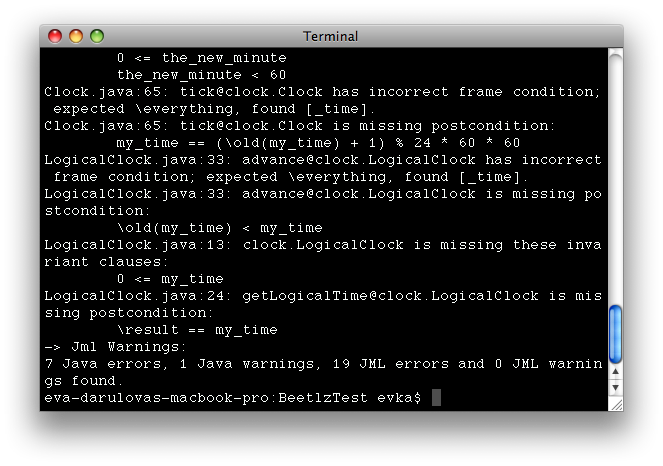
\includegraphics[width=\textwidth]{check_console}
\caption{Consistency check results in the command-line version}
\label{checkscreenshot}
\end{figure}


\section{User options}
In order for the tool to be effective and usable, it has to provide the user with ways to customise it for a particular project. At times, one may be more interested in the `big picture' and would, for example, only like to make sure that the model includes all classes and does not want the output to be filled up by small assertion details, another time exactly these may be of interest. For this, the following user options are available:
\begin{description}
\item[Error filtering] By default, all errors will be shown, but each type (error or warning) may be filtered out.
\item[No JML or no Java] The consistency check may be limited to Java only constructs and thus ignore all assertion related elements. Note that using this switch will also ignore all defined model fields and methods and ghost fields. Or otherwise one may limit the error messages to JML-related ones only as well.
\item[Pure BON] In a few places, the tool extends the original BON definition (for details, see \autoref{relations}) and if desired the option exists to use the unaltered BON definition.
\item[Source selection] For a consistency check, the source input is assumed to be the `correct' version of the project so that errors are related to the target files. By default this selection is made based on the latest time stamp of the files, so that most recently edited files are assumed `correct'. In general, this selection will be appropriate, but it can be overridden if desired. 
\item[Nullity checks] As mentioned previously, BON and JML have different default assumptions when it comes to \lstinline@null@ references. This can potentially cause a great amount of (unwanted) error messages. This option will disregard these.
\item[Skeleton generation] If the skeleton code option is selected, no consistency check will be performed, instead the source input will be printed in its corresponding representation in the target language. In this case the source option may be useful to force the tool to print in the correct programming language. Optionally, a directory can be supplied, so that the result will not be printed to standard output but to one or more files. 
\item[User Settings file] Beetlz currently includes mappings for BON basic types to the most common types in Java (see \autoref{recognizedtypes}). In many cases, the user will want to extend this list by custom types and can do so by supplying Beetlz with a text file with these mappings. Additionally, mappings for class and feature/method names can be specified as well, enabling the user to give hints to the tool to make the consistency check as accurate as possible. 
\item[JML specs] By default, OpenJML internal specification files are used to parse and check Java input files. If the user wishes to use their own, potentially more complete ones, he can do so using this option.
\end{description} 

\section{Eclipse plugin}
The Eclipse plugin includes the same functionality as the command line version but is extended by a more convenient user interface. Before the tool is used, the user has the opportunity to set custom settings on the Preferences page, which is found on the Eclipse platform by selecting \lstinline{Window->Preferences}. The options selected are stored for future use. 
Resources selected in the \lstinline{Package view} (that is projects or individual files) are then recursively searched for recognised file types and the results are presented in the following ways:
\begin{itemize}
\item Problem markers in the text editor mark the errors directly in the source files where they occur. Tool tip messages describe the nature of the errors.
\item The errors are also listed in the \lstinline{Problems} view. Different problems are assigned different types (Java errors, Java warnings, JML errors, JML warnings and General notes), so that one can use the sorting and filtering options in the \lstinline{Problems view} to customise which errors are shown.
\item The errors are additionally also printed in their command-line form to the \lstinline{Console}, from where they can be copied to the clipboard as needed.
\end{itemize}
A screenshot of the \lstinline{Preferences} page and the different presentations of errors can be found in \autoref{preferencesscreenshot} and \autoref{eclipseerrors} respectively.
\begin{figure}[h]
\begin{center}
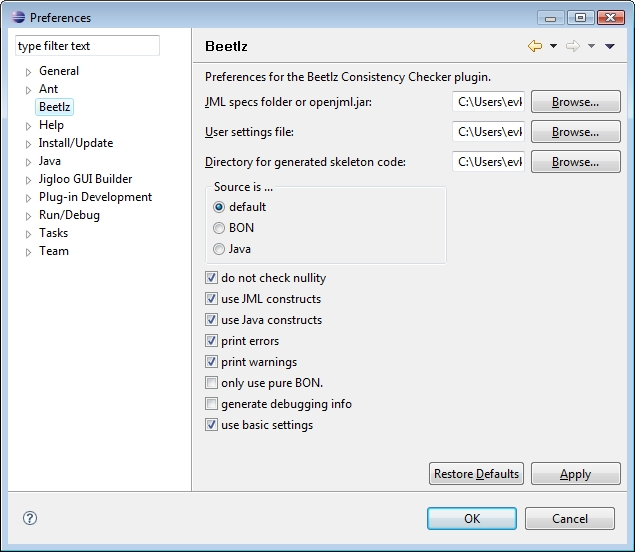
\includegraphics[totalheight=0.8\textwidth]{preferences_screenshot}
\caption{Beetlz \lstinline{Preferences} page}
\label{preferencesscreenshot}
\end{center}
\end{figure}

\begin{figure}[h]
\begin{center}
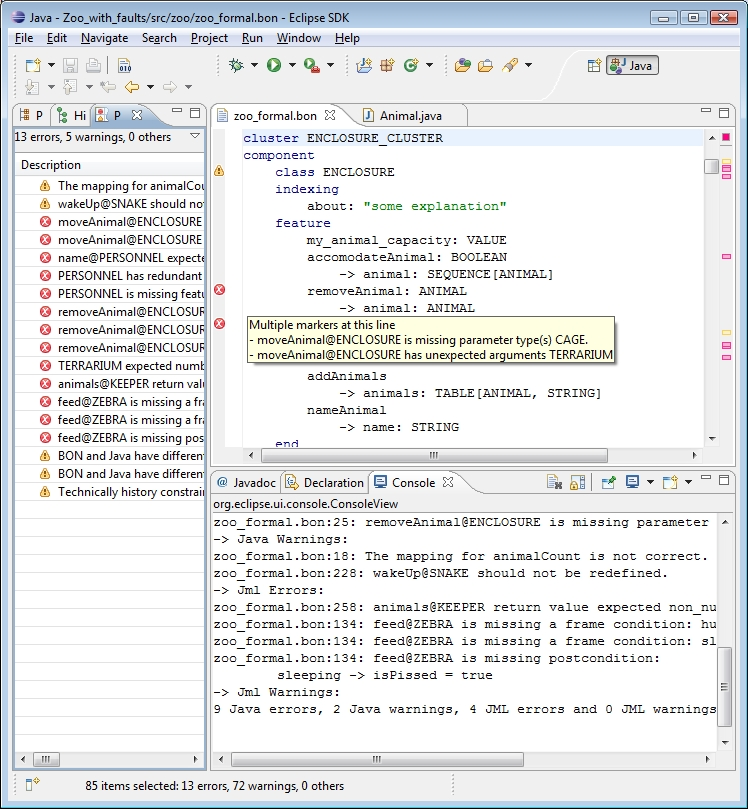
\includegraphics[totalheight=\textwidth]{eclipse_errors}
\caption{Presentation of errors in Eclipse}
\label{eclipseerrors}
\end{center}
\end{figure}

Note: The Eclipse plugin version is currently not available on Mac OS X. This is due to the fact that the Beetlz tool requires Java version 1.6. The Eclipse platform on Mac OS X itself can currently only be run with Java 1.5 as some of its libraries have not yet been ported from 32 bit versions and thus do not work with the 64 bit Java 1.6 JVM. This issue is know and currently being resolved. This does not affect the command-line version. 

\section{Testing}
Testing has been done continuously throughout development. For this type of application, creating automated tests would take a considerable amount of time, possibly more that the development of the application itself, so it was opted for doing this manually by creating input files and checking the output produced by actually reading it. Since no application is likely to feature all types of recognised errors possible, a suitable test program has been written and continuously adapted as needed. The tool was tested for functionality, that is for the actual consistency checking, and also for robustness by providing illegal input and making sure it reacts `gracefully'. The test program developed and used is included in a fault-free and in a faulty version in the released distribution and is ready to be used for demonstrations. \\ 
In the final step, Beetlz was tested on two external applications: 
\begin{enumerate}
\item The Clock example~\cite{chalin06jml} includes four short classes written in Java and in BON complete with annotations. Hence it is perfect to test the consistency checking functionality. The initial test was satisfactory, in that the BON - Java check was completely successful and the BON - JML highlighted only one major and a few minor bugs. 
\item The IDebug example\cite{idebug09repository} is a project in development for a Java logging system. Initially, informal BON charts have been prepared, but not updated with time, so that this program presents a good opportunity to test the BON skeleton code generation. The first test run was successful and has produced a full formal BON specification of the project.
\end{enumerate}
Due to the complexity of the BON, Java and JML languages and their relations, it is not possible to exhaustively test the application. Due to continuous testing during development, basic functionality is provided for and actual utilisation by users will uncover any missed details, as well as further desired functionality.

\section{Localisation}
The Beetlz tool and plugin have been fully localised, so that all messages that the user may see can be presented in any language. The current distribution includes an English and a German language file, with English being the default configuration. The language is chosen automatically based on the language setting of the Java Virtual Machine and can be changed manually by the VM argument \lstinline@-Duser.language=de@. An example of where user language dependent items appear is the menu, which can be seen in English and in German in \autoref{menueng} and \autoref{menuger}.
\begin{figure}[h]
\begin{center}
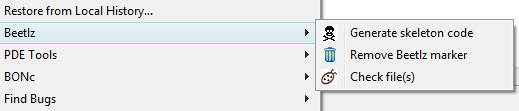
\includegraphics[width=\textwidth]{beetlz_eng_menu}
\caption{Beetlz menu in English}
\label{menueng}
\end{center}
\end{figure}

\begin{figure}[h]
\begin{center}
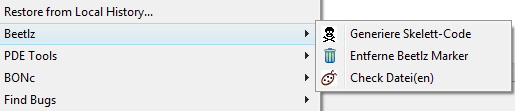
\includegraphics[width=\textwidth]{beetl_menu_ger}
\caption{Beetlz menu in German}
\label{menuger}
\end{center}
\end{figure}

\section{Limitations}
The theoretical discussion in \autoref{relations} has revealed several instances, where a BON model cannot be mapped entirely to its implementation; some operators do not have an equivalent in the other notation (see \autoref{operators}) or indeed entire clauses cannot be mapped. In some cases it is possible to circumscribe the expression and include in a different format in the consistency check. Since these procedures are in general quite complex and time-consuming, they have not been attempted in the current Beetlz distribution.

Furthermore, as mentioned before (see \autoref{jmlrelations}), light-weight specifications are assumed by the tool. If this is not the case, that is if heavy-weight specification cases are used to annotate methods, the tool will still work correctly, however it will only consider the first specification case that appears and ignore all others. If this is not accurate enough, it can be side stepped by desugaring the JML annotations first, thus creating one specification case and then running the tool.

Limitations can also be found when generating skeleton code. Some elements do not have an exact mapping so that resulting code may not compile. Additionally, only elements present are translated, so that for example Java import statements or package information will not appear. The generated code is thus meant to be reviewed by the user and corrected where necessary.
 
However, these are not the only limitations as the technology used imposes restrictions itself. So for example, due to bugs in OpenJML, classes cannot be placed in default packages at this point. These issues are being investigated and as soon as they are resolved in the third party software, Beetlz will work correctly with them. In the meantime the user is advised to create a package by the name `defaultpackage', which is recognised correctly by the tool.

Initially, the tool was planned to be made `efficient' by only performing a consistency check on files that have been changed since the last check. It turns out, that this cannot be achieved in a simple way. Each consistency checking run requires complete knowledge of all involved elements. Hence, if the tool were only to use changed files, it would need to store all required information between runs and retrieve it when necessary. Also, some typechecking functionality of BON and OpenJML only works correctly, if all files are supplied. Based on these difficulties and on the fact that the Beetlz tool operates sufficiently fast as is\footnote{The IDebug example with 18 classes and roughly 1000 method lines of code takes about 3 seconds on a 2.4GHz Mac.}, this feature is not implemented. 

\chapter{Conclusions and Future Work}
\label{conclusions}
Consistency checks are commonly being performed during software development as they help to identify potential bugs and errors. Most common examples are compilers and typechechers for specific languages but work has also been done on tools that check the consistency between different software models~\cite{paige07consistencycheck}, different representations within the same notation~\cite{litvak03behavioralUML} or fully integrated industrial solutions\cite{rhapsody09modelUml}. This report extends this work in that it presents a relation between the model language BON and the concrete implementation language Java. The successful partial implementation shows that an automatic consistency checking tool is indeed feasible and meaningful even if the relation is not always perfect. Surprisingly, mappings between BON and pure Java constructs prove to be more complex and more involved than relations on the assertion languages. It may also seem to the casual reader that those relations have many deficiencies, but in fact the details they are concerned with mostly turn out to be exotic and rather rare special cases. The Beetlz tool has been designed to be tolerant in those instances so that it can be readily used in software development.

This project and the experience gained from concluding it also show that BON and JML are straightforward enough to be quickly learned by anyone with average knowledge of Java. It has been suggested before to use BON for introducing more formal approaches into software engineering and in universities especially~\cite{kiniry08ninja}. By providing tool support that links BON to a very popular programming language, Beetlz is thus also suitable for promoting formal methods.

The basic relations between BON and Java are implemented and ready for use but further work remains to be done. Some concepts can only be mapped unsatisfactorily, however these relations can be corrected by extending BON further and thus customising it towards Java and other similar object oriented languages. Instances for such extensions include static access, more elaborate generics and an exact definition of client relations. Furthermore, BON dynamic charts, another possible description of a project, have been entirely disregarded in this analysis, but may prove useful when specifying a program's behaviour. Support for additional JML elements, like multiple specification cases, heavy-weight specifications or further operators will also become important if Beetlz is to be used in actual software development. Another area of improvement is the generation of skeleton code.  The current functionality works fine when used by itself, however creation of ASTs would make it possible to pass on information to other tools and thus provide more comprehensive functionality. (Currently this not possible due to limitations on third party projects but is in development).

On the theoretical side, formalising the relations between BON and Java, which at present only exist in structured English, would make a very interesting but also quite involved future project.

This project outlines how it is possible and advantageous to use a model of the software together with its implementation in a seamless manner. With added tool support, as the Beetlz tool demonstrates, updating of the model and/or the implementation is taken care of mostly automatically and thus can serve two purposes:
\begin{enumerate}
\item Encourage the use of software models in software engineering.
\item Reduce faults and misunderstandings resulting from poor communication with customers and/or team members.
\end{enumerate}
%%%% ADD YOUR BIBLIOGRAPHY HERE
\newpage
%\begin{thebibliography}{99}

\bibliographystyle{ieeetr}
\bibliography{bibliography} 

%\end{thebibliography}
\label{endpage}



\end{document}

\end{article}
